\begin{frame}{Phenomenological Models}
  \begin{quote}
    With four parameters I can fit an elephant, and with five I can make him wiggle his trunk. --- John von Neumann
  \end{quote}
  \vspace{-1ex}
  \begin{multicols}{2}
    \begin{itemize}
    \item Over-fitting is a pathology
    \item \emph{Good} subgrid models do not require re-tuning parameters
    \item Fracture
    \item Turbulence modeling
    \end{itemize}
  \end{multicols}
  \begin{quote}
    A professional problem exists %in the computational fluid dynamics community and also in the broader area of computational physics. Namely,
[...] there is a need for higher standards on the control of numerical accuracy. [...] it was impossible to evaluate and compare the accuracy of different turbulence models, since one could not distinguish physical modeling errors from numerical errors related to the algorithm and grid. [...] The Journal of Fluids Engineering {\bf will not accept for publication any paper}
% reporting the numerical solution of a fluids engineering problem
[...] that fails to address the task of {\bf systematic truncation error testing and accuracy estimation}. --- 1986
  \end{quote}
\end{frame}

{
\usebackgroundtemplate{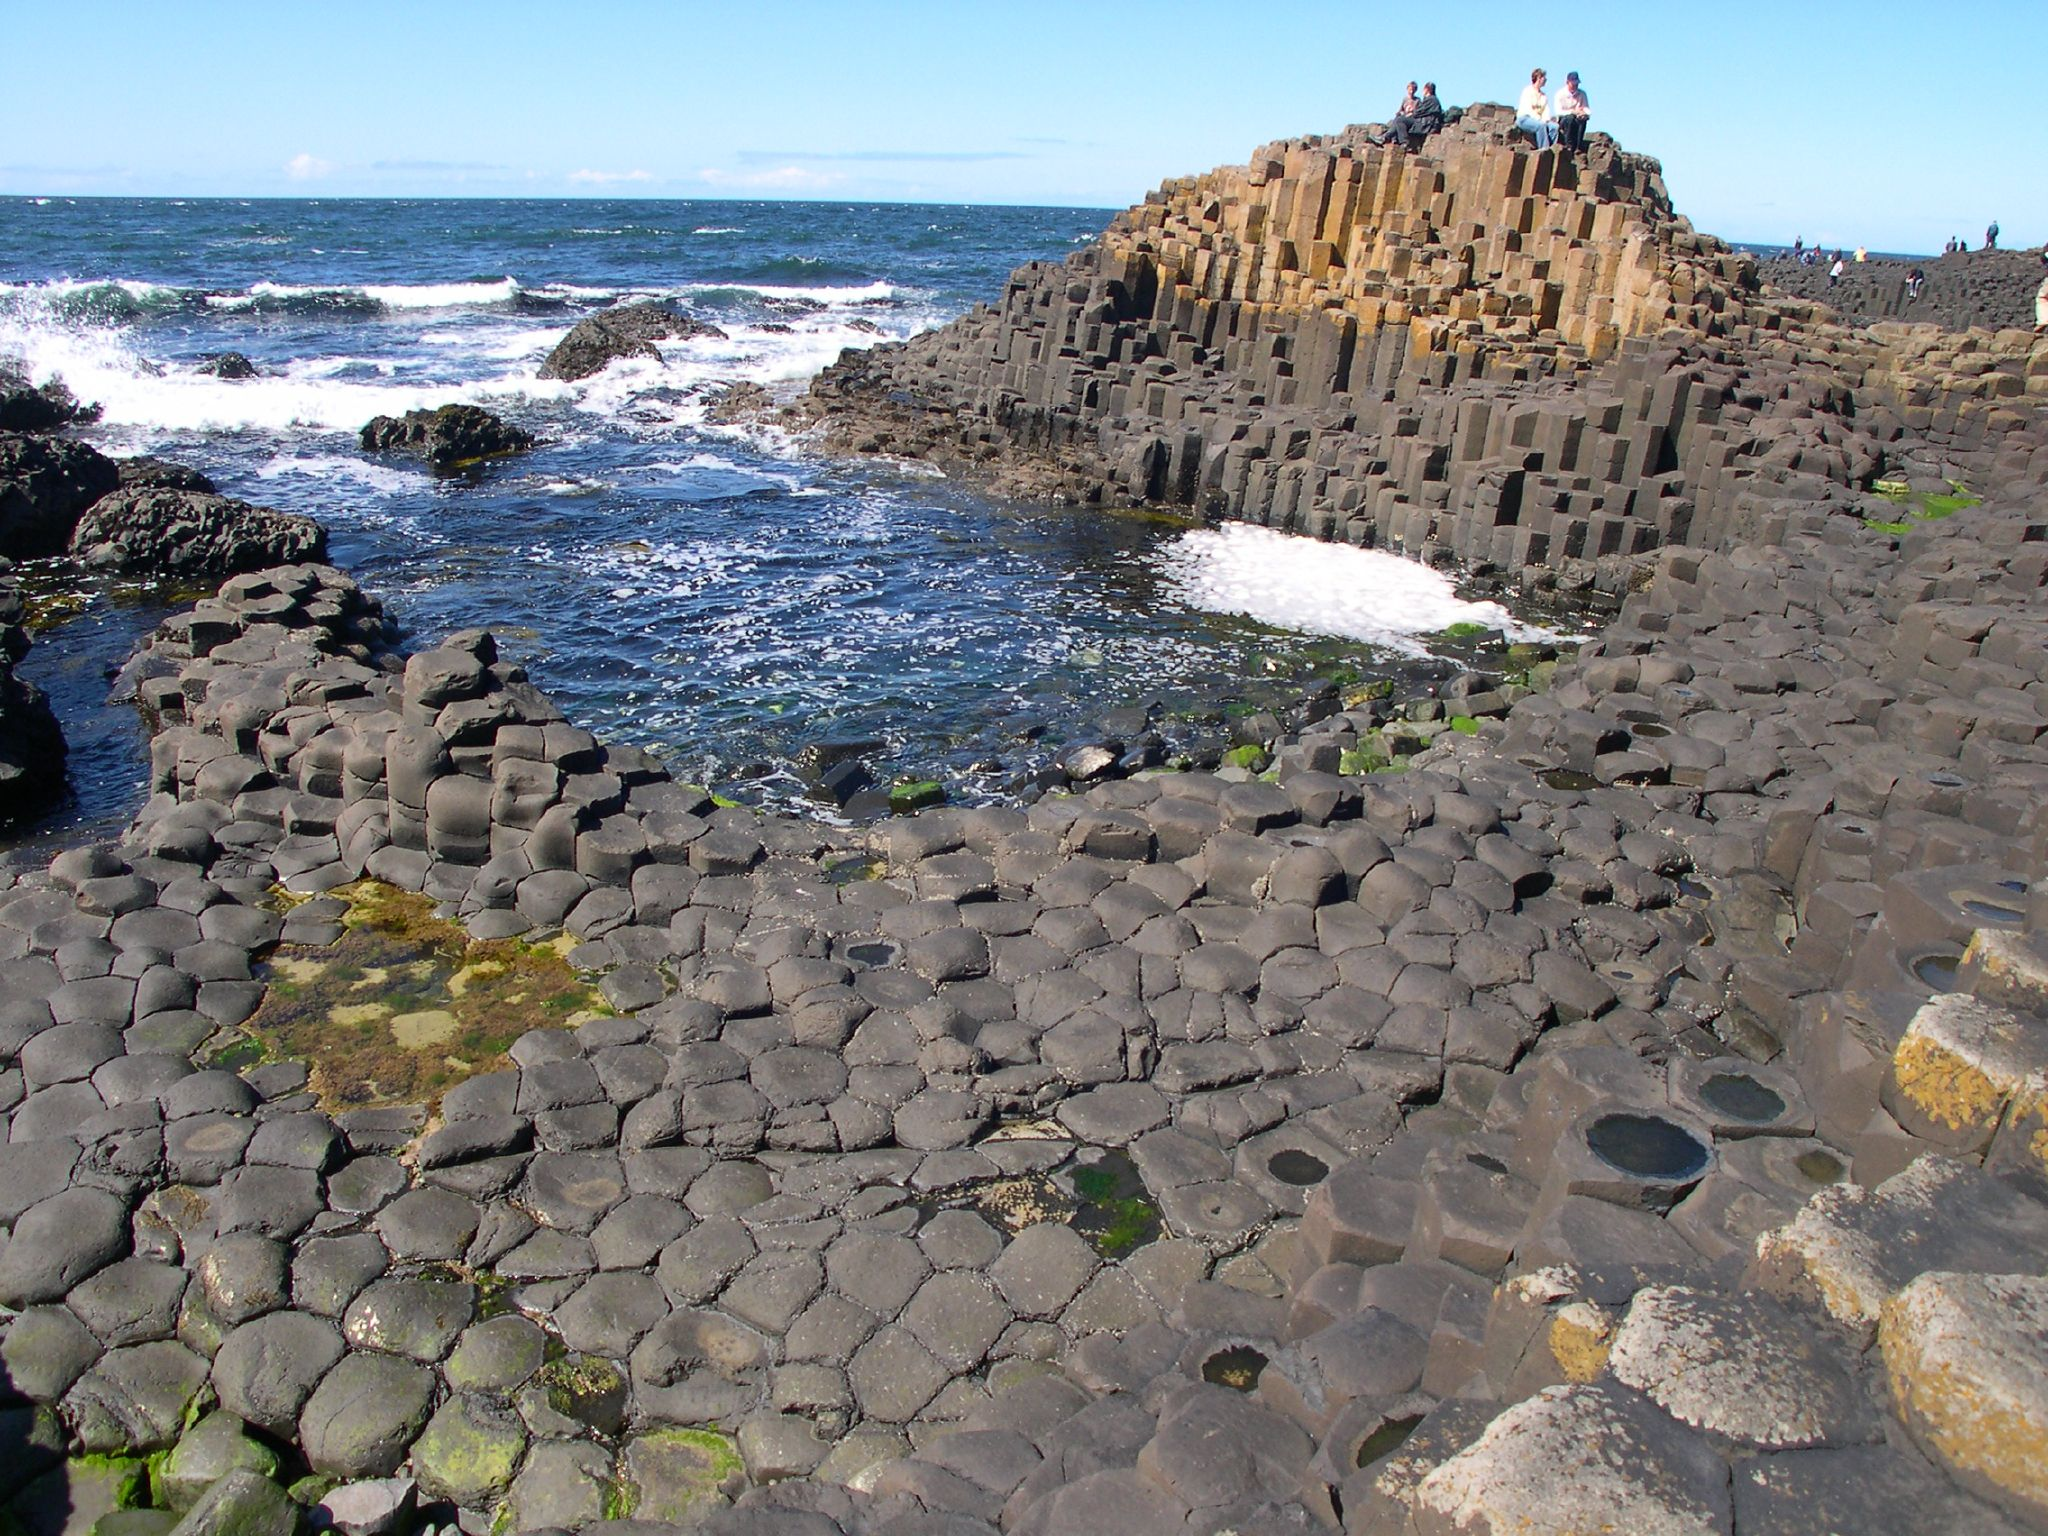
\includegraphics[width=\paperwidth]{figures/GiantsCauseway}}%
\begin{frame}{Diffusive cooling}
  \begin{textblock}{0.5}[1,0](0.99,0.1)
    \textblockcolour{black}
    \begin{itemize} \color{white} \small
    \item Pentagonal structures occur only for narrow band of thermal conditions and composition
    \item Variational (phase-field) approach reproduces thresholds without tuning [Bourdin, Francfort, Marigo]
    \end{itemize}
    %\movie{\includegraphics[width=\textwidth]{CoolingFrame.jpg}}{Cooling.mov}
    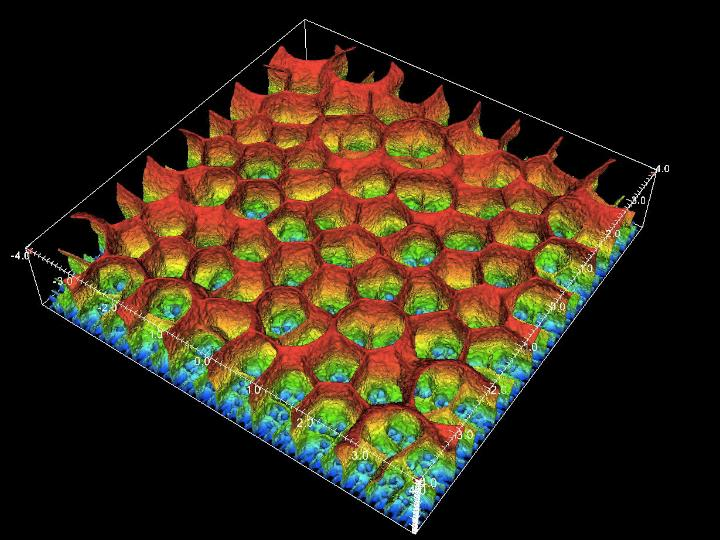
\includegraphics[width=\textwidth]{figures/BlaiseCoolingFrame.jpg}
  \end{textblock}
  % \begin{columns}
  %   \begin{column}{0.5\textwidth}
  %   \end{column}
  %   \begin{column}{0.5\textwidth}
  %   
  %   \end{column}
  % \end{columns}
\end{frame}
}
